
\chapter{The Serre Equations}
\label{chp:Serreeqns}
In this chapter the Serre equations are introduced and their relevant properties are presented.

The Serre equations are a system of partial differential equations that describe the free-surface waves of fluids whose motion is dominated by gravitational forces. They are an approximation to the Euler equations \cite{Euler-1755-274}; describing waves in shallow water when the characteristic depth of the water $h_0$ is much smaller than the characteristic wavelength of the waves $\lambda_0$ so that the shallowness parameter $ \sigma = h_0 / \lambda_0  \ll 1 $. Typically, water is considered to be shallow when $\sigma  \le  1/ 20$ \cite{Sorenson-2006}. Tsunamis and storm surges are shallow water waves as the typical ocean depth in which they occur is $4km$ and both can have wavelengths up to $100km$ long.

The Serre equations for one-dimensional flows over horizontal beds were first derived by \citet{Serre-F-1953-857} using asymptotic expansion. They were later derived using depth integration by \citet{Su-Gardener-1969-536}. They are equivalent to the Green-Naghdi equations \cite{Green-Naghdi-1976-237} derived using the theory of directed fluid sheets. The Serre equations were then extended to spatially varying bathymetry by \citet{Seabra-Santos-etal-1987-117}. 

The Serre equations are fully non-linear and thus applicable across the entire range of wave amplitudes $a_0$ which are usually characterised using the non-linearity parameter $\epsilon = a_0 / h_0$. The fluid described by the Serre equations possesses a non-hydrostatic pressure distribution and is dispersive in nature, as are real fluids. Furthermore, the dispersion relationship of linear waves of the Serre equations well approximates the linear wave theory for the Euler equations \cite{Barthelemy-2004-315}. For these reasons the Serre equations are considered one of the best approximate water wave models up to wave-breaking \cite{Bonneton-Lannes-2009-16601,Bonneton-etal-2011-1479}. 

In this chapter we present the one-dimensional Serre equations and a reformulation of these equations into conservation law form with a source term. We then present the relevant properties of the Serre equations and introduce the forced solutions which are used to assess the validity of the numerical methods. Finally, the contribution of my research \cite{Pitt-2018-61} to understanding the behaviour of steep gradients in the free-surface for the Serre equations is summarised. 

\section{The One-Dimensional Serre Equations}
In this thesis we take the Serre equations as derived from the depth-integration approach \cite{Su-Gardener-1969-536,Seabra-Santos-etal-1987-117}. Given the extent of the literature already available for the derivation of these equations we will only introduce the relevant quantities and present the equations. The one-dimensional Serre equations describe the behaviour of unsteady free surface fluid flow for an inviscid fluid with a constant density $\rho$ neglecting wave-breaking. In this thesis we will also neglect bottom friction effects as they can be incorporated into our methods after solving the Serre equations without them. 

The primitive variables of the Serre equations are the height $h(x,t)$ of a column of fluid above the stationary bed profile given by $b(x)$ and the horizontal velocity $u(x,t)$ of the column of fluid which are all shown in Figure \ref{fig:WaterModel}. The stage $w(x,t) = h(x,t) + b(x)$ gives the absolute location of the free surface. Additionally, to relate the primitive variables of the Serre equations to the intuitive variables of the Euler equations we introduce the horizontal velocity $u'(x,z,t)$ and the vertical velocity $v'(x,z,t)$ of a fluid particle.

%v hat, u hat for particle
\begin{figure}
	\centering
	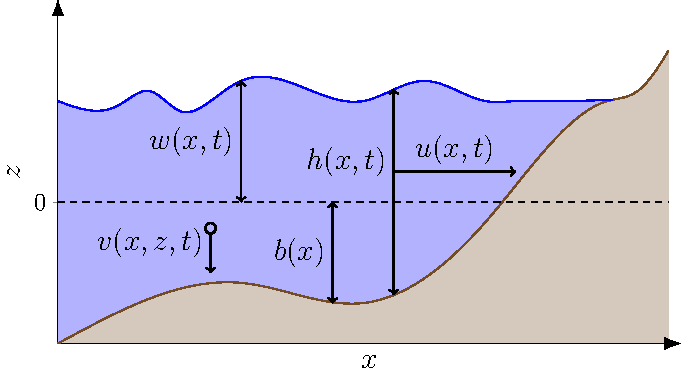
\includegraphics[width=0.8\textwidth]{./chp2/figures/SerreModel.pdf}
	\caption{Diagram demonstrating a free surface flow (\squareF{blue}) over a bed (\squareF{brown!80!black}) where $w(x,t)$ is the absolute location of the free surface, $v'(x,z,t)$ is the vertical velocity of a particle of fluid, $u'(x,z,t)$ is the horizontal velocity of a particle of fluid, $h(x,t)$ is the height of a column of fluid, $u(x,t)$ is the horizontal velocity of a column of fluid and $b(x)$ is the stationary bed profile.}
	\label{fig:WaterModel}
\end{figure}

The derivation is similar to that of the Shallow Water Wave Equations (SWWE) \cite{Liggett-1994}. In particular, we assume that the horizontal velocity of a particle of fluid $u'(x,z,t)$ inside a column of fluid equals the horizontal velocity of the column of fluid $u(x,t)$. By integrating the conservation of mass equation for an invscid fluid with a no-slip condition at the bed we obtain the distribution of the vertical velocity of a fluid particle throughout a column of fluid \cite{Zoppou-2014}
\begin{equation}
v'(x,z,t) = u \frac{\partial b}{\partial x} - (z - b) \frac{\partial u}{\partial x}.
\label{eqn:VertVelSerre}
\end{equation}
Unlike the SWWE the vertical velocity of fluid particle in the Serre equations is not zero throughout the depth of water. This leads to a non-hydrostatic pressure distribution on the fluid particles which is derived by integrating the conservation of vertical momentum equation given by the Euler equations with a no-slip condition at the bed \cite{Zoppou-2014}
\begin{equation}
\label{eqn:SerrePress}
 p'(x,z,t) = \underbrace{ \rho g \left(h + b - z\right)}_{\text{hydrostatic pressure}} + \rho \left(h + b - z\right) \Psi + \frac{1}{2} \rho \left(h^2 - \left[z - b \right]^2\right) {\Phi }
\end{equation} 
where
\begin{subequations}
	\begin{align}
	{ \Psi }  &= \dfrac{\partial b}{\partial x}\left(\dfrac{\partial u}{\partial t} + u\dfrac{\partial u}{\partial x} \right)  + u^2\dfrac{\partial^2 b}{\partial x^2}, \label{eqn:SerreeqnPsi} 
	\\ \nonumber \\
	{ \Phi }  &= \dfrac{\partial u }{\partial x} \dfrac{\partial u}{\partial x} -u \dfrac{\partial^2 u}{\partial x^2}  - \dfrac{\partial^2 u}{\partial x \partial t} . \label{eqn:SerreeqnPhi} 
	\end{align}
	\label{eqn:FullSerreNonConVarDef}
\end{subequations}
The hydrostatic pressure term $\rho g \left(h + b - z\right)$ is the pressure due to the weight of water above the fluid particle. The non-hydrostatic pressure terms are a consequence of the non-zero vertical velocity which modifies the underlying hydrostatic pressure distribution causing dispersion of waves in the free surface. 

Integrating the Euler equations \cite{Su-Gardener-1969-536,Zoppou-2014} over the entire depth with a no-slip condition at the bed, a free surface condition at the free surface, the vertical velocity relation \eqref{eqn:VertVelSerre} and the pressure distribution \eqref{eqn:SerrePress} we obtain the Serre equations
\begin{subequations}
	\begin{align}
	&\frac{\partial h}{\partial t} + \dfrac{\partial (uh)}{\partial x} = 0,  \label{eqn:FullSerreNonConMass} \\ \nonumber \\
	&\dfrac{\partial (uh)}{\partial t} + \dfrac{\partial}{\partial x} \left ( u^2h + \dfrac{gh^2}{2} + \dfrac{h^2}{2}{\Psi} + \dfrac{h^3}{3}{ \Phi }  \right )  +  \dfrac{\partial b}{\partial x} \left (gh +   h \Psi + \dfrac{h^2}{2}{ \Phi }  \right ) = 0	\label{eqn:FullSerreNonConMome}
	\end{align}
	\label{eqn:FullSerreNonCon}
\end{subequations}
which are depth integrated approximations to the conservation of mass and horizontal momentum equations of the Euler equations.
When $\Phi = \Psi = 0$ the Serre equations reduce to the SWWE where the vertical velocity is zero over the depth, the pressure distribution is hydrostatic and there is no dispersion. 

Due to the presence of the $\Phi$ and $\Psi$ terms the Serre equations are more difficult to solve analytically and numerically than the SWWE. The primary reason for this is that whilst the SWWE are hyperbolic the Serre equations are neither hyperbolic nor parabolic. Furthermore, the Serre equations are not in conservation law form due to the presence of temporal derivatives in $\Phi$ and $\Psi$, although they are derived from conservation equations. 

For a horizontal bed $\partial b / \partial x = 0$, $\Psi = 0$ and so the Serre equations reduce to
\begin{subequations}
	\label{eqn:FullSerreNonConHorizbed}
	\begin{align}
	\label{eqn:FullSerreNonConMassHorizbed}
	&\frac{\partial h}{\partial t} + \dfrac{\partial (uh)}{\partial x} = 0, \\ \nonumber \\
	\label{eqn:FullSerreNonConMomeHorizbed}
	&\dfrac{\partial (uh)}{\partial t} + \dfrac{\partial}{\partial x} \left ( u^2h + \dfrac{gh^2}{2} + \dfrac{h^3}{3}{ \Phi }  \right ) = 0.
	\end{align}
\end{subequations}	
For a horizontal bed the Serre equations are more challenging to solve analytically and numerically than the SWWE. 

\subsection{Alternative Form}
A major hurdle for developing numerical methods for the Serre equations is the presence of the temporal derivative in $\Phi$ and $\Psi$ \eqref{eqn:FullSerreNonConVarDef}. By rewriting the Serre equations and introducing a new conserved quantity $G$ \cite{Hank-etal-2010-2034,Zoppou-2014,Li-2014-169} the Serre equations can be written in conservation law form with a source term
\begin{subequations}
	\label{eqn:FullSerreCon}
	\begin{align}
	& \frac{\partial h}{\partial t} + \dfrac{\partial (uh)}{\partial x} = 0 ,\label{eqn:FullSerreConMass}  \\ \nonumber \\
	\begin{split}
	\label{eqn:Serreconsconmom}
	\frac{\partial G}{\partial t}  + \frac{\partial}{\partial x} \left( {u} G + \frac{gh^2}{2} - \frac{2}{3}h^3 \left[\frac{\partial {u}}{\partial x}\right]^2 + h^2 {u}\frac{\partial {u}}{\partial x}\frac{\partial b}{\partial x} \right) \\ \\ +  \underbrace{\frac{1}{2}h^2 {u} \frac{\partial {u}}{\partial x} \frac{\partial^2 b}{\partial x^2}  - h {u}^2\frac{\partial b}{\partial x}\frac{\partial^2 b}{\partial x^2} + gh\frac{\partial b}{\partial x} } _{\text{source term}} = 0
	\end{split}
	\end{align}
\end{subequations}
with
\begin{equation}
\label{defn:SerreEqnConservedQuantity1}
G =  {u}h \left(1 + \frac{\partial h}{\partial x}\frac{\partial b}{\partial x} + \frac{1}{2}h\frac{\partial^2 b}{\partial x^2} + \left[\frac{\partial b}{\partial x}\right]^2 \right) - \frac{\partial}{\partial x}\left(\frac{1}{3}h^3  \frac{\partial {u}}{\partial x}\right)
\end{equation}
which resembles $h$ multiplied by the irrotationality \cite{Choi-Camassa-1999-1,Carter-Cienfuegos-2011-259}.

This conservation law form makes the Serre equations well suited to be numerically solved using the finite volume method for the conservation of $h$ and $G$ equations, provided one can solve for the remaining primitive variable $u$ given $h$, $G$ and $b$.

For a horizontal bed $\partial b / \partial x = 0$ the conservation law form of the Serre equations using the new quantity $G$ is
\begin{subequations}
	\label{eqn:FullSerreConHorizBed}
	\begin{align}
	&\frac{\partial h}{\partial t} + \dfrac{\partial (uh)}{\partial x} = 0, \label{eqn:FullSerreConMassHorizBed} \\  \nonumber \\
	&\frac{\partial G}{\partial t}   + \frac{\partial}{\partial x} \left( {u} G + \frac{gh^2}{2} - \frac{2}{3}h^3 \left[\frac{\partial {u}}{\partial x}\right]^2 \right) = 0 \label{eqn:SerreconsconmomHorizBed}\\ \nonumber 
	\end{align}
	with
	\begin{align}
	&G =  {u}h  - \frac{\partial}{\partial x}\left(\frac{1}{3}h^3  \frac{\partial {u}}{\partial x}\right). \label{defn:SerreEqnConservedQuantity1HorizBed}
	\end{align}
\end{subequations}


\section{Properties}
The Serre equations possess a number of desirable properties for the modelling of water waves; in particular their conservation of fundamental quantities and dispersion relation. If a numerical method accurately approximates the Serre equations then the numerical method should reproduce the conservation and dispersion properties of the Serre equations. Furthermore, the numerical method should accurately reproduce the analytic solutions of the Serre equations. In this thesis the conservation and dispersion properties and the analytic solutions of the Serre equations are used to assess the veracity of numerical methods. 

%To complement the available analytic solutions, the Serre equations are modified to force certain solutions using a source term, which are called forced solutions. These forced solutions will be used to assess the validity of the numerical methods for a wider array of flow scenarios then possible given the limited number of analytic solutions currently available for the Serre equations.
%
%Finally the results of \citet{Pitt-2017-1725} for the behaviour of the Serre equations in the presence of steep gradients are summarised. These results demonstrate that the developed numerical method is robust in the presence of steep gradients; one of the main objectives of the thesis. 

\subsection{Conservation Properties}
A quantity is conserved if the total amount of a quantity $q$ in a closed system remains constant through time.
\begin{defn}
	\label{defn:TotalAmmountab}
	The total amount of a quantity $q$ in a system occurring on the interval $[a,b]$ at time $t$ is
	\begin{equation*}
	\mathcal{C}_q(t) = \int_{a}^{b} q(x,t)\, dx.
	\end{equation*}
\end{defn}
Using this notation conservation of a quantity $q$ implies that $\mathcal{C}_{q}(0) = \mathcal{C}_{q}(t)$ for all $t$. 

Integrating the Serre equations in both non-conservation law form \eqref{eqn:FullSerreNonCon} and conservation law form \eqref{eqn:FullSerreCon} for a closed system we get that $h$, $uh$ and $G$ are conserved by the Serre equations. Additionally, the Green-Naghdi equations \cite{Green-Naghdi-1976-237} which are equivalent to the Serre equations for one-dimensional flows were derived by conserving the energy
\begin{equation*}
	\mathcal{H}(x,t) = \frac{1}{2} \left( gh\left(h + 2b\right) + hu^2  + \frac{h^3}{3} \left[\frac{\partial u}{\partial x}\right]^2 + u^2h\left[\frac{\partial b}{\partial x}\right]^2 - uh^2 \frac{\partial u}{\partial x} \frac{\partial b}{\partial x}  \right).
	\label{eqn:Hamildef}
\end{equation*}
Therefore, the one-dimensional Serre equations should also conserve $\mathcal{H}$. The energy $\mathcal{H}$ is the sum of the gravitational potential energy
\[\frac{1}{2}\int_{b}^{h +b} gz \; dx = \frac{1}{2}gh\left(h + 2b\right),\]
the horizontal kinetic energy
\[\frac{1}{2}\int_{b}^{h +b} (u')^2 \; dx = \frac{1}{2}hu^2\]
and the vertical kinetic energy
\[\frac{1}{2}\int_{b}^{h +b} (v')^2 \; dx = \frac{1}{2} \left(\frac{h^3}{3} \left[\frac{\partial u}{\partial x}\right]^2 + u^2h\left[\frac{\partial b}{\partial x}\right]^2 - uh^2 \frac{\partial u}{\partial x} \frac{\partial b}{\partial x} \right)\]
for a column of fluid.
Where the vertical velocity of a fluid particle $v'$ for the Serre equations is given by \eqref{eqn:VertVelSerre}. For horizontal beds $\mathcal{H}$ is the Hamiltonian of the Serre equations \cite{Li-Y-2002}.
 
For the system to be closed the flux terms of the equations for $h$ and $uh$ \eqref{eqn:FullSerreNonCon} at the boundaries must cancel and the integral of the source term over the domain must vanish.

\subsection{Dispersion Properties}
The dispersion properties are studied by linearising the Serre equations with a horizontal bed, assuming periodic wave solutions and then deriving a relationship between the frequency $\omega$ and the wave number $k$ of these solutions. For the Serre equations the dispersion relation \cite{Li-2014-169} is
\begin{equation}
\label{eqn:DispersionRelation}
\omega^\pm = Uk \pm k \sqrt{gH} \sqrt{\frac{3}{\left(kH\right)^2 + 3}}
\end{equation}
where $U$ and $H$ are the mean velocity and height of the fluid respectively. For the dispersion relation two wave frequencies $\omega^+$ and $\omega^-$ are possible for each wavenumber allowing for downwind and upwind travelling waves respectively. \citet{Barthelemy-2004-315} compared this dispersion relation to the dispersion relation given by the linear theory for water waves and demonstrated its utility when $k$ is small. However, when $k$ is large the difference between the dispersion relation of the Serre equations and that of the linear water wave theory increases. 
%The dispersion relation of the Serre equations can be modified by introducing additional terms to reduce this difference \cite{Barthelemy-2004-315}, but such modifications are beyond the scope of this thesis.


From the dispersion relation \eqref{eqn:DispersionRelation} the phase velocity $v_p^\pm = \omega^\pm / k$ and the group velocity $v_g^\pm = \partial \omega^\pm / \partial  k$ can be written in terms of the wave number as
	\begin{equation*}
	\label{eqn:WaveVelocitiesPhase}
	v_p^\pm = U \pm \sqrt{gH}\sqrt{\frac{3}{\left(kH\right)^2 + 3}},
	\end{equation*}
	\begin{equation*}
	\label{eqn:WaveVelocitiesGroup}
	v_g^\pm = U \pm \sqrt{gH} \left(\sqrt{\frac{3}{\left(kH\right)^2 + 3}} \mp \left(kH\right)^2 \sqrt{\frac{3}{\left(\left[kH\right]^2 + 3 \right)^3}}\right).
	\end{equation*}
Since both the phase and group velocities depend on the wave number, waves of different wavelengths travel at different speeds indicating that the Serre equations describe dispersive waves.

Fortunately, the phase velocity and the group velocity of waves are bounded, since as $k \rightarrow 0$ then $v_p^\pm$ and $v_g^\pm \rightarrow U \pm \sqrt{gH}$ and as $k \rightarrow \infty$ then $v_p^\pm$ and $v_g^\pm \rightarrow U$. Therefore, we have that
\begin{subequations}
\begin{align}
&U - \sqrt{gH} \le v_p^- \le U \le v_p^+ \le U + \sqrt{gH}, \\
&U - \sqrt{gH} \le v_g^- \le U \le v_g^+ \le U + \sqrt{gH}
\end{align}
\label{eqn:WaveVelocitiesBound}
\end{subequations}
so that the speed of waves in the Serre equations are bounded by the speed of waves in the SWWE.

\subsection{Analytic Solutions}
Currently few analytic solutions have been discovered for the Serre equations. There is a travelling wave solution for a horizontal bed \cite{El-etal-2006} and the trivial stationary lake at rest solution for arbitrary bathymetry.


\subsubsection{Solitary Travelling Wave Solution}
The Serre equations admit a travelling wave solution that propagates at a constant speed without deformation due to a balance between the non-linear and dispersive effects. Unlike the Euler equations this travelling wave solution has a closed form
\begin{subequations}
	\begin{align}
	&h(x,t) = a_0 + a_1\text{sech}^2\left(\kappa \left[x - ct\right]\right), \\  \nonumber \\
	&u(x,t) = c\left(1 - \dfrac{a_0}{h(x,t)}\right), \\
	&b(x) = 0
	\end{align}
	\label{eqn:Solitondefhub}
\end{subequations}
with
\begin{align*}
&\kappa = \dfrac{\sqrt{3a_1}}{2 a_0\sqrt{\left(a_0 + a_1\right)}}, \\ \\
&c = \sqrt{g(a_0 + a_1)}.
\end{align*}
From these equations the total amounts of $h$ \eqref{eqn:SolitonConservationh}, $uh$ \eqref{eqn:SolitonConservationuh}, $G$ \eqref{eqn:SolitonConservationG} and $\mathcal{H}$ \eqref{eqn:SolitonConservationH} at $t=0s$ can be derived. These expressions are provided in Appendix \ref{app:ConQuant}.

This solitary wave solution has an amplitude of $a_1$, an infinite wavelength and propagates on water $a_0$ deep. It is one member of a family of smooth periodic travelling wave solutions \cite{El-etal-2006}. Note that these solitary wave solutions are not true solitons, due to their inelastic collisions with one another \cite{Dutykh-etal-2013-761}. 

This analytic solution can only be reproduced with the appropriate order of accuracy if all terms of the Serre equations with a horizontal bed \eqref{eqn:FullSerreConHorizBed} are adequately approximated by the numerical method. Furthermore, since this solution is maintained by a balance between non-linear and dispersive effects it tests the balance of these effects in the numerical method. Therefore, this analytic solution is a good test for assessing the accuracy of numerical methods for solving the Serre equations with a horizontal bed \eqref{eqn:FullSerreConHorizBed}.

\subsubsection{Lake at Rest}
The lake at rest solution is a trivial stationary solution of the Serre equations that exists for all bathymetry $b(x)$. It is a consequence of a balance between the hydrostatic pressure distribution and the forcing of the bed slope. The lake at rest solution is
\begin{subequations}
	\begin{align}
	&h(x,t) = \max\left\lbrace a_0 - b(x), 0 \right\rbrace, \\
	&u(x,t) = 0 , \\
	&G(x,t) = 0 .
	\end{align}
	\label{eqn:LARdefhub}
\end{subequations}
It represents a quiescent body of water with a horizontal water surface or stage $w(x,t) = h(x,t) + b(x)$ over any bathymetry. With the maximum function included in the water depth to allow for dry regions of the bed when $b(x) > a_0$. We write these quantities in terms of $b(x)$ as this solution holds for all bed profiles. The corresponding total amounts of $h$ and $\mathcal{H}$ can be calculated by summing their total amounts in wet regions \eqref{eqn:AppLARhwet}. While the total amounts of $u$ and $G$ are zero. The expressions to calculate the total amount of the conserved quantity over any domain are provided in Appendix \ref{app:ConQuant}. 

Since $w(x,t)$ is constant when $h> 0$ then $\partial w / \partial x = \partial h / \partial x + \partial b / \partial x = 0 $ and $u=0$ so that the Serre equations \eqref{eqn:FullSerreCon} reduce to
\begin{align*}
& \frac{\partial h}{\partial t}  = 0,  &\frac{\partial G}{\partial t}  = 0.
\end{align*}
Therefore, $G$ and $h$ are constant in time and so is $u$ and thus the solution is stationary.

For naive numerical methods of the Serre equations the hydrostatic pressure terms do not balance the bed slope terms. This causes the numerical solutions of an initially still lake to produce non-physical velocities, degrading their convergence to the solution. To combat this, modifications are made to the flux and source term approximations so that these terms do balance, leading to a so called `well-balanced' method. This analytic solution then provides a test for the effectiveness of these well-balancing modifications to the numerical methods.


\section{Forced Solutions}
%ADD SOMETHING ABOUT NOT CONSERVATIVE
The known analytic solutions of the Serre equations provide a stringent test when the bed is horizontal, as all terms in the equations are non-zero and vary in space and time. For varying bathymetry there is only the lake at rest solution where all terms are constant in time and some vanish. Therefore, the accuracy of the approximations of all terms of the Serre equations in the numerical method is not adequately assessed using only the currently available analytic solutions.

Currently the verification of the order of accuracy of the numerical methods for transient solutions with varying bathymetry requires the use of forced solutions. To do this we select some particular functions for all of the primitive quantities; $h$, $u$ and $b$ which we denote $h^*$, $u^*$ and $b^*$ respectively. To force these functions $h^*$, $u^*$ and $b^*$ to be solutions of the Serre equations \eqref{eqn:FullSerreCon} we add the terms $S_h$ and $S_G$ to obtain the forced Serre equations
\begin{subequations}
	\label{eqn:FullSerreConForced}
	\begin{align}
	& \frac{\partial h}{\partial t} + \dfrac{\partial (uh)}{\partial x} + S_{h}  = 0 ,\label{eqn:FullSerreConMassForced}  \\ \nonumber \\
	\begin{split}
	\label{eqn:SerreconsconmomForced}
	\frac{\partial G}{\partial t}  + \frac{\partial}{\partial x} \left( {u} G + \frac{gh^2}{2} - \frac{2}{3}h^3 \left[ \frac{\partial {u}}{\partial x} \right]^2 + h^2 {u}\frac{\partial {u}}{\partial x}\frac{\partial b}{\partial x} \right) \\ \\ + \frac{1}{2}h^2 {u} \frac{\partial {u}}{\partial x} \frac{\partial^2 b}{\partial x^2}  - h {u}^2\frac{\partial b}{\partial x}\frac{\partial^2 b}{\partial x^2} + gh\frac{\partial b}{\partial x} + S_{G} = 0
	\end{split}
	\end{align}
\end{subequations}
where
\begin{align*}
&  S_{h} = -\frac{\partial h^*}{\partial t} - \dfrac{\partial (u^*h^*)}{\partial x} ,  \\ \nonumber \\
\begin{split}
S_{G} = -\frac{\partial G^*}{\partial t}  - \frac{\partial}{\partial x} \left( {u}^* G^* + \frac{g\left[h^*\right]^2}{2} - \frac{2}{3}\left[h^*\right]^3 \left[\frac{\partial {u}^*}{\partial x}\right]^2 + \left[h^*\right]^2 {u^*}\frac{\partial {u}^*}{\partial x}\frac{\partial b^*}{\partial x} \right) \\ \\ - \frac{1}{2}\left[h^*\right]^2 {u}^* \frac{\partial {u}^*}{\partial x} \frac{\partial^2 b^*}{\partial x^2}  + h^* {\left[u^*\right]}^2\frac{\partial b^*}{\partial x}\frac{\partial^2 b^*}{\partial x^2} - gh^*\frac{\partial b^*}{\partial x}.
\end{split}
\end{align*} 
These forced Serre equations are then numerically solved by solving the Serre equations \eqref{eqn:FullSerreCon} with the analytic values of $S_{h}$ and $S_{G}$ given $h^*$, $u^*$ and $b^*$. So that, the only error present in the numerical solutions of the forced Serre equations is the error produced by the numerical methods used to solve the Serre equations.

Note that since the choice of the forced solutions $h^*$, $u^*$ and $b^*$ is arbitrary the solutions of the forced Serre equations need not be conservative or retain any properties of the underlying Serre equations. 

%These forced solutions do not retain properties 

%%%[][][][]
\section{Behaviour in the Presence of Steep Gradients}
To ensure that the developed numerical methods are robust, their capability to handle initial condition problems with quantities possessing discontinuities must be tested. One group of these initial condition problems that has been of particular interest to the water wave community is the dam-break problem \cite{El-etal-2006,Hank-etal-2010-2034,Mitsotakis-etal-2014,Mitsotakis-etal-2017,doCarmo-etal-2018-404}. The dam-break problem consists of an intially still body of water with a discontinuous jump in its surface between two depth values. So that

\begin{subequations}
	\begin{align}
	&h(x,0) =\left\lbrace \begin{array}{l r}
	h_l & x < x_0 \\
	h_r & x \ge x_0,
	\end{array} \right. \\
	&u(x,0) = 0 , \\
	&G(x,0) = 0 , \\
	&b(x) = 0
	\end{align}
	\label{eqn:DBdefhub}
\end{subequations} 
where $h_l$ and $h_r$ are the water depth to the left and right of $x_0$ respectively. 

Currently, these dam-break problems \eqref{eqn:DBdefhub} have no known analytic solutions for the Serre equations. However, some insight into the behaviour of the evolution of these initial condition problems has been gained from asymptotic \cite{El-etal-2006} and linear \cite{Dougalis-etal-2007} analyses. 

There have also been a number of numerical solutions to dam-break problems presented in the literature \cite{El-etal-2006,Hank-etal-2010-2034,Mitsotakis-etal-2014,Mitsotakis-etal-2017,doCarmo-etal-2018-404} which have used a variety of numerical methods. Some of these numerical methods could not handle discontinuous initial conditions \cite{El-etal-2006,Mitsotakis-etal-2014,Mitsotakis-etal-2017,doCarmo-etal-2018-404} and so smooth approximations to the initial conditions \eqref{eqn:DBdefhub} were employed. The variety of numerical approaches has lead to different conclusions about the behaviour of the evolution of dam-break problems in the Serre equations in the literature. To resolve these differences a comprehensive review of a particular dam-break problem with a variety of numerical methods and smoothing of the initial conditions was performed \cite{Pitt-2018-61}. 

The convergence and conservation properties of many numerical solutions of the first-, second- and third-order finite difference volume methods as well as two second-order finite difference methods were investigated \cite{Pitt-2018-61}. All the numerical solutions affirmed the existence of a previously unreported behaviour of the Serre equations in the presence of steep gradients over short time spans. This new behaviour was justified using the convergence of the numerical solutions to one another as the resolution of the method increased. Since this convergence was observed for all high-order accurate methods; the likelihood that this new behaviour was a result of a particular quirk of the method was small. Indicating that this behaviour is representative of the true solution of the Serre equations in the presence of steep gradients. This new behaviour was then reproduced by a reviewer with their own independently constructed method and by the second-order finite element volume method described in this thesis. 

The analytic solution of the Serre equations to the dam-break problem is not currently known. These numerical solutions \cite{Pitt-2018-61} currently provide the best approximation to the solution of the Serre equations to the dam-break problem over short time spans. Furthermore, these results demonstrate the effect of smoothing the initial conditions and low grid resolutions on the observed behaviours. This allows others to appropriately choose the smoothness of the initial conditions and the resolution of their numerical method.

The relevant results garnered from the asymptotic \cite{El-etal-2006} and linear \cite{Dougalis-etal-2007} analyses for the evolution of the dam-break problem are presented here, followed by a summary of the numerical results \cite{Pitt-2018-61}, which constituted a significant portion of my research. Since the rest of this thesis is focused around the development and validation of the second-order finite element volume method and the paper \cite{Pitt-2018-61} is focused on other methods, we provide only a brief summary of this work in this thesis.

\subsubsection{Asymptotic and Linear Results}
The asymptotic analysis of \citet{El-etal-2006} used Whitham modulation to study the evolution of dispersive shock waves of the Serre equations as $t\rightarrow \infty$. Because, a dispersive shock wave is generated in the evolution of the dam-break problem in the Serre equations; these results are very useful. In particular, they provide a relationship between the initial heights of the dam-break problem $h_l$ and $h_r$ and the amplitude $A^+$ and speed $S^+$ of the leading wave in the resulting dispersive wave train. These quantities are obtained by solving
\begin{subequations}
	\begin{align}
	&\frac{\Delta}{\left(A^+ + 1\right)^{1/4}} - \left(\frac{3}{4 -  \sqrt{A^+ + 1}}\right)^{21/10} \left(\frac{2}{1 + \sqrt{A^+ + 1}}\right)^{2/5} = 0,	\label{eqn:Aplusdef} \\  \nonumber \\
	&S^+ = \sqrt{g \left(A^+ + 1\right)}	\label{eqn:Splusdef}
	\end{align}
	\label{eqn:ELWhitMod}	
\end{subequations}
where
\begin{equation*}
\Delta = \frac{1}{4 h_r}\left(\sqrt{\dfrac{h_l}{h_r}} + 1\right)^2.
\end{equation*}
These expressions were found to agree well with numerical simulations provided that $\Delta < 1.43$ \cite{El-etal-2006}.

For the linearised Serre equations we obtain the dispersion relation \eqref{eqn:DispersionRelation} from which the phase and group velocities can be determined \eqref{eqn:WaveVelocitiesBound}. The negative and positive branches of the phase and group velocities are separated, implying that there should be a separation of the upwind and downwind parts of the dispersive wave-train \cite{Dougalis-etal-2007}. Therefore, the structure of dispersive shock waves of the Serre equations should be two separate dispersive wave trains.


\subsubsection{Numerical Solutions for the Smoothed Dam-break Problem}
To resolve the differences present in the literature a variety of numerical methods were used to solve the most common class of smoothed versions of the dam-break problem initial conditions \eqref{eqn:DBdefhub}. This was termed the smoothed dam-break problem and is given by
\begin{subequations}
	\begin{align}
	&h(x,0) = h_r + \dfrac{h_l - h_r}{2} \left(1 +  \tanh\left(\dfrac{x_0 - x}{\alpha}\right) \right), \\
	&u(x,0) = 0 , \\
	&G(x,0) = 0 , \\
	&b(x) = 0
	\end{align}
	\label{eqn:SmoothDB}
\end{subequations}
where $\alpha$ controls the width of the transition from $h_l$ to $h_r$ and thus the steepness of the initial gradient in the water surface. Most of the numerical simulations were focused on solutions for $h_l = 1.8m$, $h_r = 1m$ and $x_0 = 500m$ with a final time of $t=30s$. The smoothing parameter $\alpha$ and the resolution of the methods were varied to investigate their influence on the observed behaviour of the numerical solution. Four structures were observed in the numerical solutions; the non-oscillatory structure, the flat structure, the node structure and the growth structure. Numerical solutions at $t=30s$ for the mentioned $h_l$, $h_r$ and $x_0$ values demonstrating examples of the observed structures are shown in Figure \ref{fig:DBExAll}. 
\begin{figure}
	\centering
	\begin{subfigure}{0.5\textwidth}
		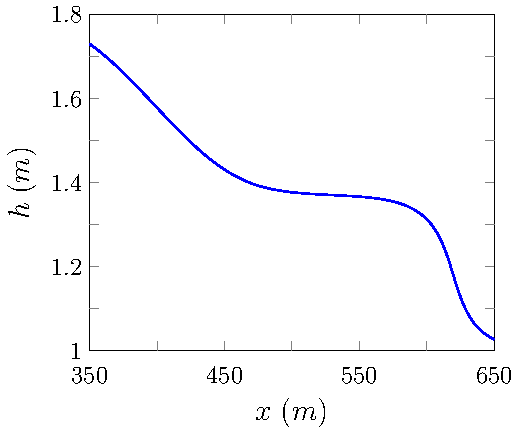
\includegraphics[width=\textwidth]{./chp2/figures/DamBreakStruct/1.pdf}
		\subcaption{Non-Oscillatory Structure}
		\vspace{0.5cm}
	\end{subfigure}%
	\begin{subfigure}{0.5\textwidth}
		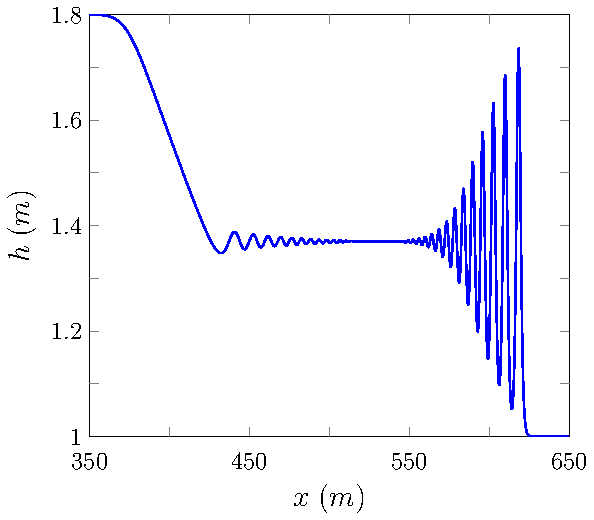
\includegraphics[width=\textwidth]{./chp2/figures/DamBreakStruct/6.pdf}
		\subcaption{Flat Structure}
		\vspace{0.5cm}
	\end{subfigure}
	\begin{subfigure}{0.5\textwidth}
		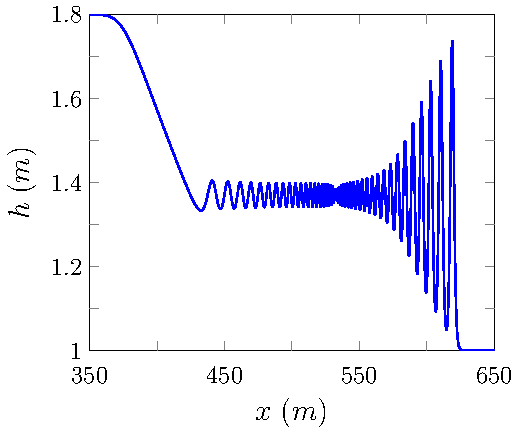
\includegraphics[width=\textwidth]{./chp2/figures/DamBreakStruct/9.pdf}
		\subcaption{Node Structure}
		\vspace{0.5cm}
	\end{subfigure}%
	\begin{subfigure}{0.5\textwidth}
		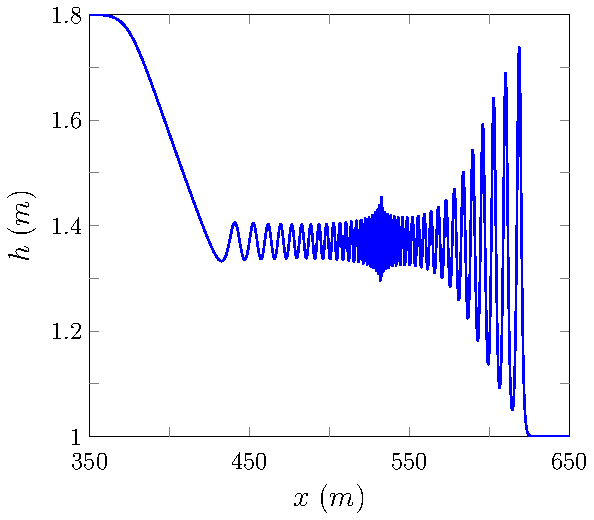
\includegraphics[width=\textwidth]{./chp2/figures/DamBreakStruct/20.pdf}
		\subcaption{Growth Structure}
		\vspace{0.5cm}
	\end{subfigure}
	\caption{Examples of the different structures observed in numerical solutions to the smoothed dam-break problem \eqref{eqn:SmoothDB} displayed by \citet{Pitt-2018-61}.}
	\label{fig:DBExAll}
\end{figure}

The growth structure was previously not reported in the literature. The growth structure was consistently observed in numerical solutions of the smoothed dam-break problem for high-order accurate methods as $\alpha$ and the grid resolution were increased. Therefore, the growth structure represents the true structure of the solution of the Serre equations for the dam-break problem with the corresponding $h_l$ and $h_r$ values at $t=30s$. This conclusion was supported by measuring the convergence of the numerical solutions to one another and observing the conservation of the conserved quantities. 

The finite difference volume methods introduced diffusive errors caused by their flux approximation, so that the amplitude and number of oscillations in the dispersive wave train increased as the resolution increased. While the finite difference methods introduce dispersive errors decreasing the amplitude and number of oscillations in the dispersive wave train as the resolution was increased. Therefore, the numerical solutions of both classes of methods serve as upper and lower bounds on the amplitude and number of oscillations in the dispersive wave train. These bounds further demonstrated that the observed growth structure best represented the true solution of the Serre equations to this dam-break problem. 

The observation of other behaviours at $t=30s$ is caused by; small $\alpha$ values which overly smooth the initial conditions, low-order numerical methods introducing large diffusive errors and low numerical resolutions which cannot resolve the high frequency waves observed in the growth structure. These structures exist on a spectrum where the severity of these effects determine the observed behaviour. So that, the most severe damping effects produced the non-oscillatory structure and the least severe effects produced the growth structure. These effects explained the observations of different structures previously present in the literature \cite{El-etal-2006,Hank-etal-2010-2034,Mitsotakis-etal-2014,Mitsotakis-etal-2017}. 

The differences in the observed structures are primarily driven by the different internal structures of the dispersive shock wave, so that for the flat, node and growth structure in Figure \ref{fig:DBExAll} the front of the dispersive wave trains are indistinguishable. Therefore, the results of numerical solutions that have not resolved all the internal structure present in the growth structure still agree well with the Whitham modulation results \eqref{eqn:ELWhitMod} of \citet{El-etal-2006}.

The amplitude of waves at the centre of the growth structure decays over time, resulting in the observation of the flat structure when $t$ is large. These results agree with the linear argument put forth by \citet{Dougalis-etal-2007}. This indicates that for smaller times the non-linear terms of the Serre equations play a significant role in the evolution of steep gradients. While for long times the linear terms are dominant and thus a separation of the dispersive wave trains is observed. 

\medskip

In this chapter the Serre equations and their relevant properties were given. The forced Serre equations were introduced and a summary of the main results for the evolution of steep gradients in the free surface was provided. We now will describe the finite element volume method, whose development was a primary objective of the thesis. 
